\section[Loss Functions, Optimization, and Initialization]{Loss Functions, Optimization, and Initialization}

\begin{frame}{Loss Functions, Optimization, and Initialization}
	Now that the gradient backpropagation algorithm holds no secrets for you, we have left to tackle three key architectural aspects that we have set aside until now:
	
	\begin{itemize}
		\item \textbf{Loss functions}: We have mathematically propagated the error gradient $\delta$ across layers, but we have not yet defined how this initial error vector is explicitly computed.
		\pause
		\item \textbf{Optimization}: We briefly outlined how to \textit{update} the structural weight and bias terms via gradient descent once the partial derivatives are resolved, but much remains to be discussed regarding advanced optimization.
		\pause
		\item \textbf{Initialization}: Our assumptions regarding the initial state of weights and biases have remained highly evasive, stating only that they are initialized \textit{randomly}. We will see \textit{precisely} how this initialization must be executed to ensure numerical stability.
	\end{itemize}
\end{frame}

\subsection[Loss Functions]{Loss Functions}

\begin{frame}{Loss Functions}
	In this section, we will introduce specialized loss functions tailored for the supervised learning frameworks encountered so far:
	\begin{itemize}
		\item For linear regression problems: the \textbf{squared error} function.
		\item For binary classification problems: the \textbf{binary cross-entropy} function.
		\item For multi-class classification problems: the \textbf{categorical cross-entropy} function.
	\end{itemize}
	We will also formulate the analytical entries required to seed the gradient backpropagation pipeline by computing the derivatives of these objectives.
\end{frame}

\begin{frame}{Naming Conventions and Rigor}
	\begin{itemize}
		\item The \textbf{loss function} $L$ computes a localized error metric unitaire, evaluated on a single, isolated observation.
		\item The \textbf{cost function} aggregates individual loss metrics across the entire training dataset. The most common aggregation operator is the empirical mean. In our introduction, we formally defined this objective as the empirical risk $R_n$.
		\item The \textbf{error} $e$ evaluates to a single global scalar across all $n$ training instances; it represents the output of the cost function.
	\end{itemize}
	\vspace{0.5cm}
	\begin{equation*}
		e = \frac{1}{n} \sum_{i=1}^{n} L\left(y^{(i)}, \hat{y}^{(i)}\right)
	\end{equation*}
\end{frame}

\subsection[Loss Function for Regression]{Loss Function for Regression}

\begin{frame}{Squared Errors for Regression}
	The squared error framework was introduced in Chapter 1 as the structural foundation of empirical learning:
	\begin{equation*}
		L\left(y^{(i)}, \hat{y}^{(i)}\right) = \left(y^{(i)} - \hat{y}^{(i)}\right)^2
	\end{equation*}
	This is the exact loss framework used to derive classical linear regression.
	\pause
	\begin{equation*}
		e = \frac{1}{n} \sum_{i=1}^n \left(y^{(i)} - \hat{y}^{(i)}\right)^2
	\end{equation*}
	\pause
	The initial vector gradient $\delta = \frac{\partial{e}}{\partial{\hat{Y}}} \in \mathcal{M}_{n,1}(\R)$ is analytically resolved as follows:
	\begin{equation*}
		\delta = 
		\begin{pmatrix}
			\frac{\partial{e}}{\partial{\hat{y}^{(1)}}} \\[5pt]
			\frac{\partial{e}}{\partial{\hat{y}^{(2)}}} \\[5pt]
			\vdots \\
			\frac{\partial{e}}{\partial{\hat{y}^{(n)}}} \\
		\end{pmatrix}
		=
		\begin{pmatrix}
			\frac{2}{n} \left(\hat{y}^{(1)} - y^{(1)}\right) \\
			\frac{2}{n} \left(\hat{y}^{(2)} - y^{(2)}\right) \\
			\vdots \\
			\frac{2}{n} \left(\hat{y}^{(n)} - y^{(n)}\right)
		\end{pmatrix}
		= \frac{2}{n} \left(\hat{Y} - Y\right)
	\end{equation*}
\end{frame}

\begin{frame}{Loss Function for a Regression Problem}
	\begin{block}{Loss Function for a Regression Problem}
		Given a continuous regression target matrix $Y \in \mathcal{M}_{n,1}(\R)$ and the neural network predictions $\hat{Y} \in \mathcal{M}_{n,1}(\R)$, the global scalar error $e \in \R$ evaluated across $n$ samples is given by:
		\begin{equation*}
			e = \frac{1}{n} \sum_{i=1}^n \left(y^{(i)} - \hat{y}^{(i)}\right)^2 = \frac{1}{n} \left(Y - \hat{Y}\right)^T \left(Y - \hat{Y}\right)
		\end{equation*}
		The partial derivative of this cost $e$ with respect to the output layer predictions $\hat{Y}$ evaluates to:
		\begin{equation*}
			\frac{\partial{e}}{\partial{\hat{Y}}} = \frac{2}{n} \left(\hat{Y} - Y\right)
		\end{equation*}
		This objective function is widely known as the \textbf{Mean-Squared Error} (MSE).
	\end{block}
\end{frame}

\subsection[Loss Function for Binary Classification]{Loss Function for Binary Classification}

\begin{frame}{Binary Cross-Entropy}
	We have already encountered the mathematical structure of binary cross-entropy twice in this curriculum:
	\begin{itemize}
		\item In our initial module, when defining the optimization objective for classical \textbf{logistic regression}.
		\item In our decision trees module, where entropy was leveraged to quantify localized node \textit{purity}.
	\end{itemize}
	\pause
	Cross-entropy evaluates the average surprise experienced by our neural network model (the predicted probability distribution) when evaluated against empirical evidence (the true probability distribution). Minimizing cross-entropy minimizes the divergence between empirical observations and predicted soft probabilities. This optimization is strictly equivalent to minimizing the Kullback-Leibler divergence.
\end{frame}

\begin{frame}{Binary Cross-Entropy}
	As previously outlined, a fundamental nuance separates the pure information-theoretic definition of cross-entropy from its implementation in machine learning:
	\begin{itemize}
		\item In theoretical information theory, we observe $n$ independent trials evaluated on a \textbf{single, unique subject}: e.g., flipping a single coin whose true success probability is estimated to compute an expected surprise metric.
		\item In machine learning applications, we observe exactly \textbf{one} trial across $n$ \textbf{entirely different subjects}. Every instance possesses its own localized true label and estimated probability parameter.
	\end{itemize}
	\pause
	For a binary classification task, the structural loss function derived from cross-entropy is written as:
	\begin{equation*}
		L\left(y^{(i)}, \hat{y}^{(i)}\right) = - y^{(i)} \ln{\left(\hat{y}^{(i)}\right)} - \left(1 - y^{(i)}\right) \ln{\left(1 - \hat{y}^{(i)}\right)}
	\end{equation*}
\end{frame}

\begin{frame}{Average Binary Cross-Entropy}
	Aggregating individual cross-entropy losses across the complete set of observations yields the global scalar error term $e$:
	\begin{equation*}
		e = \frac{1}{n} \sum_{i=1}^n \left[ - y^{(i)} \ln{\left(\hat{y}^{(i)}\right)} - \left(1 - y^{(i)}\right) \ln{\left(1 - \hat{y}^{(i)}\right)} \right]
	\end{equation*}
	\pause
	The initial vector gradient $\delta = \frac{\partial{e}}{\partial{\hat{Y}}} \in \mathcal{M}_{n,1}(\R)$ evaluates as follows:
	\begin{equation*}
		\begin{aligned}
			\delta 
			&= 
			\begin{pmatrix}
				\frac{\partial{e}}{\partial{\hat{y}^{(1)}}} \\[5pt]
				\frac{\partial{e}}{\partial{\hat{y}^{(2)}}} \\[5pt]
				\vdots \\
				\frac{\partial{e}}{\partial{\hat{y}^{(n)}}} \\
			\end{pmatrix}
			= \frac{1}{n}
			\begin{pmatrix}
				-\frac{y^{(1)}}{\hat{y}^{(1)}} + \frac{\left(1 - y^{(1)}\right)}{\left(1 - \hat{y}^{(1)}\right)} \\[5pt]
				-\frac{y^{(2)}}{\hat{y}^{(2)}} + \frac{\left(1 - y^{(2)}\right)}{\left(1 - \hat{y}^{(2)}\right)} \\[5pt]
				\vdots \\
				-\frac{y^{(n)}}{\hat{y}^{(n)}} + \frac{\left(1 - y^{(n)}\right)}{\left(1 - \hat{y}^{(n)}\right)}
			\end{pmatrix} \\
			&= \frac{1}{n} \left( -Y \text{ } \oslash \text{ } \hat{Y} + \left(1_Y - Y\right) \text{ } \oslash \text{ } \left(1_Y - \hat{Y}\right)\right)
		\end{aligned}
	\end{equation*}
\end{frame}

\begin{frame}{Analytical Fusion for Gradient Propagation}
	An elegant mathematical simplification is systematically engineered into modern deep learning frameworks:
	\begin{itemize}
		\item In binary classification tasks, a smooth \textbf{logistic} sigmoid function maps raw unconstrained \textbf{logits} to bounded \textbf{probabilities}.
		\item During backward propagation, combining the derivative of the binary cross-entropy loss with the localized derivative of the logistic activation function collapses into a highly clean, linear expression.
	\end{itemize}
\end{frame}

\begin{frame}{Analytical Fusion for Gradient Propagation}
	Recall that the derivative of the logistic function can be expressed as:
	\begin{equation*}
		\sigma'(Z) = \sigma(Z) \odot \left(1_Z - \sigma(Z)\right) = \hat{Y} \odot (1_Y - \hat{Y})
	\end{equation*}
	\pause
	Consequently, by direct application of the multi-dimensional chain rule:
	\begin{equation*}
		\begin{aligned}
			\frac{\partial{e}}{\partial{Z}} 
			&= \delta \odot \sigma'(Z) \\
			&= \frac{1}{n} \left( - Y \oslash \hat{Y} + \left(1_Y - Y\right) \oslash \left(1_Y - \hat{Y}\right)\right) \odot \hat{Y} \odot (1_Y - \hat{Y}) \\
			&= \frac{1}{n} \left( - Y \odot (1_Y - \hat{Y}) + \hat{Y} \odot \left(1_Y - Y\right)\right) \\
			&= \frac{1}{n} \left( - Y \cdot 1_Y + Y \odot \hat{Y} + \hat{Y} \cdot 1_Y - \hat{Y} \odot Y \right) \\
			&= \frac{1}{n} \left( \hat{Y} - Y \right)
		\end{aligned}
	\end{equation*}
\end{frame}

\begin{frame}{Loss Function for Binary Classification Problems}
	\begin{block}{Loss Function for Binary Classification Problems}
		Given binary ground-truth labels $Y \in \mathcal{M}_{n,1}(\{0, 1\})$, unconstrained network \textbf{logits} $Z \in \mathcal{M}_{n,1}(\R)$, and the logistic sigmoid activation $\sigma$, the global empirical cost $e \in \R$ across $n$ samples is formalized as:
		\begin{equation*}
			e = \frac{1}{n} \sum_{i=1}^n \left[ - y^{(i)} \ln{\left(\sigma\left(z^{(i)}\right)\right)} - \left(1 - y^{(i)}\right) \ln{\left(1 - \sigma\left(z^{(i)}\right)\right)} \right]
		\end{equation*}
		The partial derivative of this error $e$ directly with respect to the logit vector $Z$ simplifies cleanly to:
		\begin{equation*}
			\frac{\partial{e}}{\partial{Z}} = \frac{1}{n} \left(\sigma\left(Z\right) - Y\right)
		\end{equation*}
		This combined layer objective is termed \textbf{Binary Cross Entropy (BCE) with Logits}.
	\end{block}
\end{frame}

\begin{frame}{Network Optimization for Binary Classification}
	To exploit this mathematical simplification, binary classification network architectures are optimized as follows during the training phase:
	\begin{itemize}
		\item We do \textbf{not} append an activation function onto the final output layer. The network directly evaluates raw \textbf{logits}.
		\pause
		\item The Binary Cross Entropy with Logits objective function is executed. Computing the absolute scalar cost $e$ is technically unnecessary to backpropagate gradients; the framework directly seeds the pipeline with $\frac{\partial{e}}{\partial{Z}}$. This approach is computationally faster and vastly more numerically stable.
		\pause
		\item In practice, the scalar value $e$ is still computed passively to monitor global convergence curves.
	\end{itemize}
	
	\pause
	\vspace{0.3cm}
	
	Once training is complete, a logistic sigmoid function is appended to the output layer for inference tasks to map raw \textbf{logits} back to valid \textbf{probabilities}.
\end{frame}

\begin{frame}{Squared Errors vs. Cross-Entropy for Classification}
	In practice, optimizing a multi-class classification problem via a Mean-Squared Error objective is technically feasible—after all, probabilities are real numbers, and we are simply minimizing numerical distances. However, this is highly sub-optimal:
	\begin{figure}
		\centering
		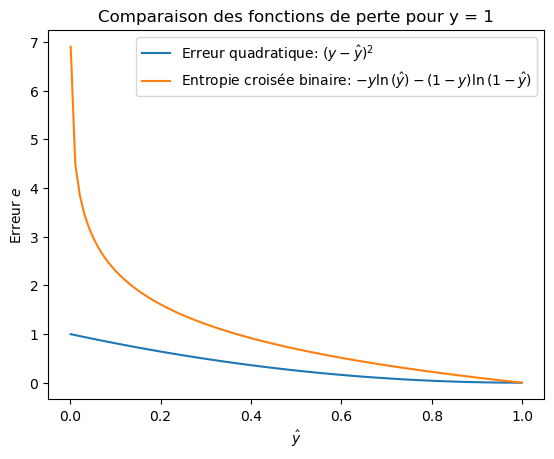
\includegraphics[width=0.4\linewidth]{Images/mse_vs_bce}
		\label{fig:mse_vs_bce}
	\end{figure}
	The gradient penalty scales drastically faster under cross-entropy than under squared errors. Cross-entropy heavily penalizes a model that confidently outputs an incorrect classification, accelerating convergence.
\end{frame}

\subsection[Loss Function for Multi-Class Classification]{Loss Function for Multi-Class Classification}

\begin{frame}{$\hat{Y}$ and $Y$ in Multi-Class Tasks}
	In a classification task spanning $K$ separate categories, the predicted soft probabilities $\hat{Y}$ and the ground-truth targets $Y$ are structured as dense matrices within $\mathcal{M}_{n, K}([0, 1])$, where $n$ represents the number of observations.
	
	\pause
	\vspace{0.5cm}
	
	For any individual observation $i$, if the true categorical class index is $k$, the target vector row is constructed as:
	
	\begin{equation*}
		\begin{cases}
			y_{j}^{(i)} = 1 & \text{if } j = k \\
			y_{j}^{(i)} = 0 & \text{if } j \ne k \\
		\end{cases} \; \text{ for } \; j = 1, 2, \cdots, K
	\end{equation*}
	
	\vspace{0.5cm}
	\pause
	
	This discrete mapping is universally known as \textbf{One-Hot Encoding}.
\end{frame}

\begin{frame}{Categorical Cross-Entropy across $K$ Classes}
	To extend binary parameters to multi-class scenarios, the structural principles remain identical:
	\begin{itemize}
		\item We replace the binary cost function with the generalized \textbf{categorical cross-entropy} objective.
		\item We swap out the single univariant logistic curve for the multivariate \textbf{softmax} operator.
		\item The training framework fuses the activation and loss steps into a single block to ensure mathematical stability.
	\end{itemize}
\end{frame}

\begin{frame}{Categorical Cross-Entropy across $K$ Classes}
	The generalized single-sample formulation of categorical cross-entropy is defined as:
	\begin{equation*}
		L\left(y^{(i)}, \hat{y}^{(i)}\right) = -\sum_{k=1}^K y_k^{(i)} \ln{\left(\hat{y}_k^{(i)}\right)}
	\end{equation*}
	\pause
	Setting $K = 2$ confirms that this expression collapses directly back into our binary cross-entropy framework:
	\begin{equation*}
		\begin{aligned}
			L\left(y^{(i)}, \hat{y}^{(i)}\right) 
			&= -\sum_{k=1}^2 y_k^{(i)} \ln{\left(\hat{y}_k^{(i)}\right)}
			= - y_{1}^{(i)} \ln{\left(\hat{y}_{1}^{(i)}\right)} - y_{2}^{(i)} \ln{\left(\hat{y}_{2}^{(i)}\right)} \\
			&= - y_{1}^{(i)} \ln{\left(\hat{y}_{1}^{(i)}\right)} - \left(1 - y_{1}^{(i)}\right) \ln{\left(1 - \hat{y}_{1}^{(i)}\right)}
		\end{aligned}
	\end{equation*}
\end{frame}

\begin{frame}{Average Categorical Cross-Entropy}
	Accumulating individual single-sample cross-entropy metrics across the complete dataset yields the global scalar cost $e$:
	\begin{equation*}
		e = \frac{1}{n} \sum_{i=1}^n \sum_{k=1}^K - y_k^{(i)} \ln{\left(\hat{y}_k^{(i)}\right)}
	\end{equation*}
	\pause
	The initial output gradient matrix $\delta = \frac{\partial{e}}{\partial{\hat{Y}}} \in \mathcal{M}_{n,K}(\R)$ is structured as follows:
	\begin{equation*}
		\delta 
		= 
		\begin{pmatrix}
			\frac{\partial{e}}{\partial{\hat{y}_1^{(1)}}} & \frac{\partial{e}}{\partial{\hat{y}_2^{(1)}}} & \cdots & \frac{\partial{e}}{\partial{\hat{y}_K^{(1)}}} \\[5pt]
			\frac{\partial{e}}{\partial{\hat{y}_1^{(2)}}} & \frac{\partial{e}}{\partial{\hat{y}_2^{(2)}}} & \cdots & \frac{\partial{e}}{\partial{\hat{y}_K^{(2)}}}\\[5pt]
			\vdots & \vdots & \cdots & \vdots \\
			\frac{\partial{e}}{\partial{\hat{y}_1^{(n)}}} & \frac{\partial{e}}{\partial{\hat{y}_2^{(n)}}} & \cdots & 
			\frac{\partial{e}}{\partial{\hat{y}_K^{(n)}}}\\[5pt]
		\end{pmatrix}
	\end{equation*}
\end{frame}

\begin{frame}{Average Categorical Cross-Entropy}
	Evaluating the localized scalar components within this gradient matrix yields:
	\begin{equation*}
		\delta_{i,k} = \frac{\partial{e}}{\partial{\hat{Y}_{i,k}}} = - \frac{1}{n} \frac{y_k^{(i)}}{\hat{y}_k^{(i)}}
	\end{equation*}
	\pause
	Expressed compactly in clean tensor notation, the output gradient matrix is written as:
	\begin{equation*}
		\delta = \frac{\partial{e}}{\partial{\hat{Y}}} = - \frac{1}{n} Y \oslash \hat{Y}
	\end{equation*}	
\end{frame}

\begin{frame}{The Softmax Activation Function}
	Recall the mathematical formulation of the softmax operator evaluated at the network's output layer:
	\begin{equation*}
		\operatorname{softmax}(z_j) = \frac{e^{z_j}}{\sum_{k=1}^{K} e^{z_k}} \; \forall \; j = 1, 2, \cdots, K
	\end{equation*}
	\pause
	This multivariate operator introduces three profound structural differences compared to univariant activation functions:
	\begin{itemize}
		\item The activation output scales to a dense matrix of dimensions $(n \times K)$.
		\item The probability map resolved for an observation $i$ at class index $k$ exhibits explicit cross-talk with all $K$ dimensions of the input layer due to the denominator summation.
		\item The formal Jacobian derivative of the softmax function with respect to its inputs expands to a complex 4th-order tensor of dimensions $(n \times K \times n \times K)$.
	\end{itemize}
\end{frame}

\begin{frame}{Tensor Formulation of the Softmax Function}
	\begin{itemize}
		\item The denominator operator sums across the rows of a dense $(n \times K)$ matrix. Mathematically, this evaluates to a localized vector of dimensions $(n \times 1)$, written as: $\exp{(Z)} 1_K$.
		\pause
		\item The numerator consists of a standard matching matrix of dimensions $(n \times K)$, namely: $\exp{(Z)}$.
		\pause
		\item Linear algebra software engines utilize implicit broadcasting to compute this division. To formalize this matrix operation rigorously without broadcasting syntax, we post-multiply by $1_K^T$ to expand the dimensions into an matching $n \times K$ matrix: $\exp{(Z)} 1_K 1_K^T$.
	\end{itemize}
	The strict, unbroadcasted tensor formulation of the softmax function is thus written as:
	\begin{equation*}
		\operatorname{softmax}(Z) = \exp{(Z)} \oslash \left(\exp{(Z)} 1_K 1_K^T\right)
	\end{equation*}
\end{frame}

\begin{frame}{Derivative of the Tensor Softmax Function}
	Evaluating a 4th-order Jacobian tensor of dimensions $(n \times K \times n \times K)$ would be computationally tedious. Instead, we bypass this complex structure entirely by executing a targeted \textbf{tensor contraction} shortcut, exactly as derived in our previous module.
	
	\vspace{0.5cm}
	
	The optimization math beautifully collapses into a lean expression identical to our binary framework:
	
	\begin{equation*}
		\frac{\partial{e}}{\partial{Z}} = \frac{1}{n} \left(\hat{Y} - Y \right)
	\end{equation*}
	
	The analytical proof for this tensor contraction is available in the appendix of this course.
\end{frame}

\begin{frame}{Loss Function for Multi-Class Classification Problems}
	\begin{block}{Loss Function for Multi-Class Classification Problems}
		Given a One-Hot encoded target matrix $Y \in \mathcal{M}_{n,K}(\{0, 1\})$, network \textbf{logits} $Z \in \mathcal{M}_{n,K}(\R)$, and the multivariate \textbf{softmax} operator, the empirical cost $e \in \R$ evaluated across $n$ observations is given by:
		\begin{equation*}
			e = - \frac{1}{n} \sum_{i=1}^n \sum_{k=1}^K y_k^{(i)} \ln{\left(\hat{y}_k^{(i)}\right)}
		\end{equation*}
		The partial derivative of this error $e$ directly with respect to the logit matrix $Z$ is formulated as:
		\begin{equation*}
			\frac{\partial{e}}{\partial{Z}} = \frac{1}{n} \left(\operatorname{softmax}\left(Z\right) - Y\right)
		\end{equation*}
	\end{block}
\end{frame}

\begin{frame}{Network Optimization for Multi-Class Classification}
	Mirroring our binary strategy, multi-class architectures are optimized via logits to maximize efficiency:
	\begin{itemize}
		\item We do \textbf{not} execute an activation function on the final layer during training. The system outputs raw \textbf{logits}.
		\pause
		\item The categorical cross-entropy loss function is executed directly from logits. The execution engine computes the gradient matrix $\frac{\partial{e}}{\partial{Z}}$ directly, bypassing slow tensor evaluations.
		\pause
		\item The empirical cost $e$ is tracked in parallel to map training diagnostic curves.
	\end{itemize}
	
	\pause
	\vspace{0.3cm}
	
	Following model convergence, a softmax activation block is appended onto the output nodes for inference tasks to convert unconstrained \textbf{logits} to standard \textbf{probabilities}.
\end{frame}

\begin{frame}{Loss Function Engineering Summary}
	We now possess the complete analytical arsenal required to seed our backpropagation pipelines:
	\begin{itemize}
		\item Driven by the statistical nature of our supervised objective, we resolve the localized \textbf{initial error gradient} and mathematically \textbf{propagate} it directly through the output activation layer.
		\pause
		\item Our previous modules detailed how to route this error vector upstream through every building block of a dense architecture: the \textbf{linear affine node} and hidden layer \textbf{activation operators}.
		\pause
		\item We can now compute the exact partial derivative of the error with respect to \textbf{any structural parameter} embedded deep within the network.
		\pause
		\item We must now formalize how to intelligently \textbf{initialize} these parameter fields and \textbf{update} them during the optimization process.
	\end{itemize}
\end{frame}

\subsection[Minimization via Gradient Descent]{Minimization via Gradient Descent}

\begin{frame}{Gradient Descent Framework}
	Let $P$ denote any generic matrix parameter (weight field or bias vector) within the model architecture, defined as a tensor within $\mathcal{M}_{u,v}(\R)$. For structural bias fields, $u = 1$.
	
	\vspace{0.3cm}
	\pause
	
	The vanilla gradient descent optimization algorithm operates as follows:
	\begin{enumerate}
		\item Initialize parameter tensor states: $P$.
		\pause
		\item Execute an outer loop over sequential training \textbf{epochs} until a stopping criterion is met (e.g., maximum epoch limit, error cost falls below a threshold, or gradient stabilization).
		\pause
		\item For the complete set of observations in the training dataset:
		\begin{itemize}
			\item Compute the forward pass to resolve the global scalar cost $e$.
			\pause
			\item Execute gradient backpropagation to evaluate the partial derivatives $\nabla_P = \frac{\partial{e}}{\partial{P}}$ across all parameters $P$.
			\pause
			\item Update every parameter field: $P \leftarrow P - \alpha \nabla_P$.
		\end{itemize}
		\item Return to Step 2.		
	\end{enumerate}
\end{frame}

\begin{frame}{Batch vs. Stochastic vs. Mini-Batch Settings}
	In real-world data science, this framework is tailored based on the volume of instances processed simultaneously during each forward and backward cycle:
	\begin{itemize}
		\item If the system processes \textbf{all} available training instances simultaneously, it is termed \textbf{batch gradient descent}.
		\pause
		\item If the system processes exactly \textbf{one single} observation per update, it is termed \textbf{stochastic gradient descent} (SGD).
		\pause
		\item If the system targets a structured subset of size $m$, it is termed \textbf{mini-batch gradient descent}.
	\end{itemize}
	
	\pause
	\vspace{0.5cm}
	
	Let $m$ define the explicit mini-batch size. The total number of batch steps required to complete a single epoch is formulated as:
	\begin{equation*}
		N_{\text{batches}} = \left\lceil \frac{n}{m} \right\rceil
	\end{equation*}
	Where $\lceil \cdot \rceil$ represents the mathematical ceiling operator, rounding a real number up to the nearest integer.
\end{frame}

\begin{frame}{Batch vs. Stochastic vs. Mini-Batch Settings}
	To summarize the hyperparameter boundaries:
	\begin{itemize}
		\item \textbf{Batch gradient descent}: $m = n$.
		\item \textbf{Stochastic gradient descent}: $m = 1$.
		\item \textbf{Mini-batch gradient descent}: $1 < m < n$.
	\end{itemize}
	
	\pause
	\vspace{0.3cm}
	
	The batch size $m$ is a critical structural \textbf{hyperparameter} requiring empirical validation:
	\begin{itemize}
		\item Setting a batch volume that is too large can exceed the physical VRAM allocation capacities of hardware accelerators.
		\item Setting a batch volume that is too small slows processing speed by failing to exploit the hardware \textbf{vectorization} engineered into modern CPUs and GPUs.
		\item Engineers select batch sizes as powers of 2 (e.g., 64, 128, 256, 512) to optimize memory alignment on processing units.
	\end{itemize}
\end{frame}

\begin{frame}{Mini-Batch Gradient Descent Algorithm}
	The formalized execution loop for mini-batch optimization operates as follows:
	\begin{enumerate}
		\item Initialize parameter fields: $P_{k=0}$.
		\pause
		\item Loop over sequential training \textbf{epochs}.
		\pause
		\item For each mini-batch (typically sampled randomly) of size $m$:
		\begin{itemize}
			\item Compute the forward pass and evaluate the localized error cost $e$.
			\pause
			\item Execute gradient backpropagation to compute the current gradient step: $\nabla_P = \frac{\partial{e}}{\partial{P}}$.
			\pause
			\item Execute parameter field updates: $P_{k+1} \leftarrow P_k - \alpha \nabla_P$.
			\pause
		\end{itemize}
		\item Return to Step 2 if stopping criteria are not met.
	\end{enumerate}
\end{frame}

\begin{frame}{Stochastic Path Visualization}
	\begin{figure}
		\centering
		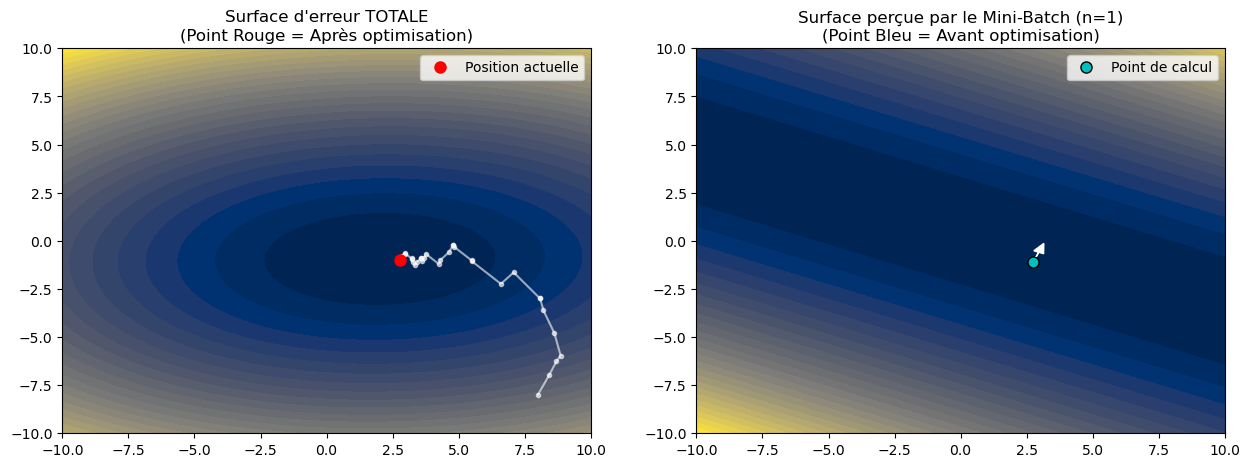
\includegraphics[height=0.35\linewidth]{Images/descente_gradient_stochastique}
		\label{fig:descente_gradient_stochastique}
		\caption*{Stochastic Gradient Descent ($m=1$)}
	\end{figure}
	Note: The spatial axes simulate an isolated two-parameter landscape ($W$ and $b$) for a minimal linear network: $\hat{Y} = X W + b$.
\end{frame}

\begin{frame}{Mini-Batch Path Visualization}
	\begin{figure}
		\centering
		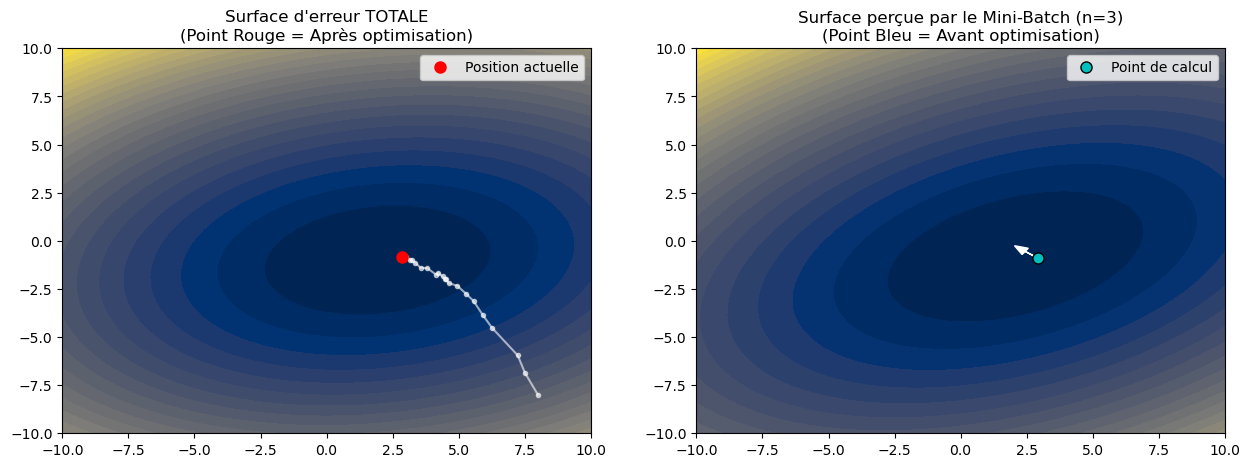
\includegraphics[height=0.35\linewidth]{Images/descente_gradient_minibatch}
		\label{fig:descente_gradient_mini_batch}
		\caption*{Mini-Batch Gradient Descent ($1 < m < n$)}
	\end{figure}
	Note: The spatial axes simulate an isolated two-parameter landscape ($W$ and $b$) for a minimal linear network: $\hat{Y} = X W + b$.
\end{frame}

\begin{frame}{Batch Path Visualization}
	\begin{figure}
		\centering
		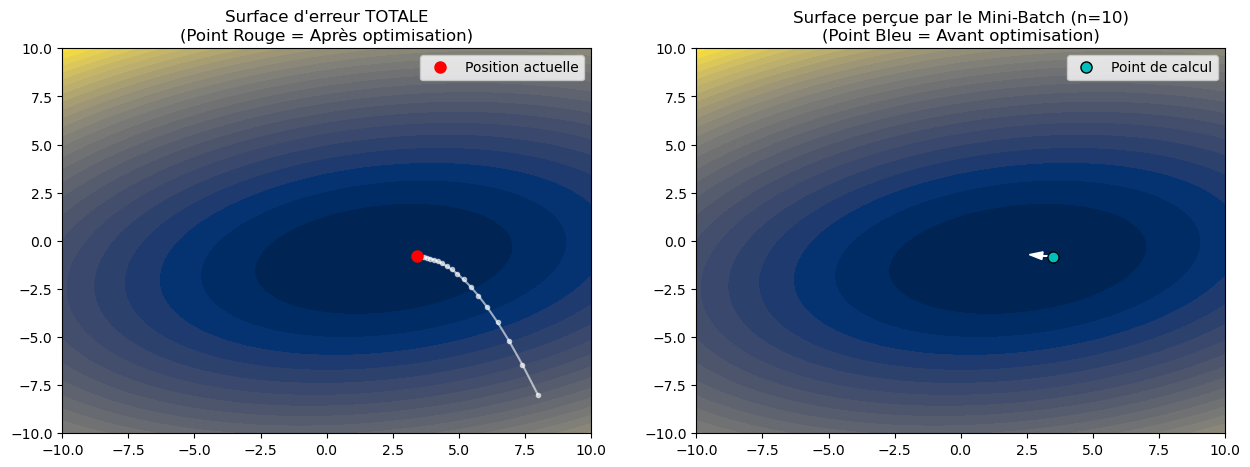
\includegraphics[height=0.35\linewidth]{Images/descente_gradient_batch}
		\label{fig:descente_gradient_batch}
		\caption*{Batch Gradient Descent ($m=n$)}
	\end{figure}
	Note: The spatial axes simulate an isolated two-parameter landscape ($W$ and $b$) for a minimal linear network: $\hat{Y} = X W + b$.
\end{frame}

\begin{frame}{The Mechanics of Cost Landscapes}
	The true mathematical geometry of the cost function landscape:
	\begin{itemize}
		\item is completely fixed for a given training dataset!
		\pause
		\item depends exclusively on the structural network architecture and the empirical data.
		\pause
		\item is completely \textbf{unknown} analytically across high-dimensional parameter spaces.
		\pause
		\item is only revealed at a \textbf{single coordinate point} during a forward pass step! The subsequent backward pass yields the localized vector slope (gradient) at that specific coordinate.
	\end{itemize}
\end{frame}

\begin{frame}{Topological Approximations and Stochastic Noise}
	When a forward pass is restricted to a small mini-batch sample, the system is effectively optimizing an \textbf{approximated} instance of the true cost landscape. The structural surface mapped by the current mini-batch fluctuates at each step. Consequently:
	\begin{itemize}
		\item The optimization \textit{path} under pure Stochastic Gradient Descent is highly \textit{noisy} and errant.
		\item The optimization \textit{path} under Mini-Batch settings is significantly \textit{smoothed}, as larger samples act as a more robust statistical proxy for the true cost function.
		\item The optimization \textit{path} under full Batch conditions is mathematically \textit{optimal}, guiding the optimizer precisely down the line of steepest global descent.
	\end{itemize}
\end{frame}

\begin{frame}{The Optimization Optimization Paradox}
	\begin{itemize}
		\item This inherent stochastic \textit{noise} can behave beneficially, helping the gradient descent optimizer escape shallow local minima or traverse saddle points. These systems remain highly vulnerable to initial parameter states.
		\pause
		\item However, an overly \textit{noisy} path introduces severe convergence delays. When training large-scale network architectures requires hours of wall-clock time on high-performance computing clusters, maximizing trajectory efficiency is paramount.
	\end{itemize}
	
	\pause
	\vspace{0.5cm}
	
	In the following slides, we will explore signal processing filtering techniques engineered to \textit{denoise} this path, combining the rapid calculation speed of mini-batch processing with the steady tracking of full batch optimization.
	
\end{frame}

\subsection[Denoising via Exponentially Weighted Moving Averages]{Denoising via Exponentially Weighted Moving Averages}

\begin{frame}{Exponentially Weighted Moving Averages}
	We introduce a classical signal processing smoothing framework: the \textbf{Exponentially Weighted Moving Average} (EWMA):
	\begin{columns}
		\begin{column}{0.5\textwidth}
			\begin{figure}
				\centering
				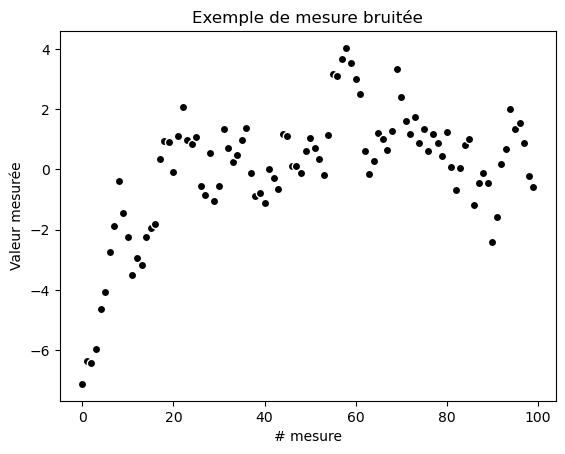
\includegraphics[width=1.0\linewidth]{Images/mesure_bruitee}
				\label{fig:mesure_bruitee}
			\end{figure}			
		\end{column}
		\begin{column}{0.5\textwidth}
			\begin{itemize}
				\item Consider a chronological sequence of fluctuating, noisy measurements.
				\item In signal processing theory, any raw \textbf{measured signal} is modeled as a composite mixture of structural \textbf{underlying information} and high-frequency stochastic \textbf{noise}.
				\item Various filtering mechanisms exist to \textit{denoise} or \textit{smooth} such data streams.
			\end{itemize}
		\end{column}	
	\end{columns}
\end{frame}

\begin{frame}{The EWMA Algorithmic Workflow}
	Let $\theta \in \R^n$ represent our raw chronological sequence of metrics, where $\theta_i$ denotes the measurement at step $i$. Let $v \in \R$ define the filtered, denoised proxy, and let $\beta \in [0, 1]$ act as the recursive memory coefficient. The standard filtering loop operates as follows:
	
	\begin{enumerate}
		\item Initialize the memory register: $v = 0$.
		\item Set a fixed configuration for the memory retention parameter $\beta$.
		\item Loop sequentially across the $n$ data steps:
		\begin{itemize}
			\item Extract the current raw observation $\theta_i$.
			\item Update the filtered proxy recursively: $v \leftarrow (1 - \beta) \theta_i + \beta v$.
			\item Repeat this block until all $n$ measurements are processed.
		\end{itemize}
	\end{enumerate}
\end{frame}

\begin{frame}{Mathematical Unrolling of the Recursive Filter}
	The recursive equation balances the influence of the \textit{current} raw metric with the aggregated historical memory of all \textit{past} states:
	\begin{equation*}
		v^{(i)} = (1 - \beta) \theta_i + \beta v^{(i-1)}
	\end{equation*}
	Setting $\beta = 0$ applies zero smoothing; the filtered output tracks the raw input signal $\theta_i$ exactly. Conversely, setting the boundary condition $\beta = 1$ freezes the filter permanently at its initialized state ($0$).
	
	\pause
	\vspace{0.5cm}
	
	Fixing $\beta = 0.9$, let us unroll the recursive loop analytically at step 3:
	\begin{equation*}
		\begin{aligned}
			v^{(3)} 
			&= (1 - \beta) \theta_3 + \beta v^{(2)} \\
			&= (1 - \beta) \theta_3 + \beta \left((1 - \beta) \theta_{2} + \beta v^{(1)} \right) \\
			&= (1 - \beta) \theta_3 + \beta (1 - \beta) \theta_{2} + \beta^2 v^{(1)} \\
			&= (1 - \beta) \theta_3 + \beta (1 - \beta) \theta_{2} + \beta^2 (1 - \beta) \theta_{1} + \underbrace{\beta^3 v^{(0)}}_{= 0}
		\end{aligned}
	\end{equation*}
\end{frame}

\begin{frame}{Mathematical Unrolling of the Recursive Filter}
	Executing the direct numerical allocation yields:
	\begin{equation*}
		\begin{aligned}
			v^{(3)} 
			&= (1 - 0.9) \theta_3 + 0.9 (1 - 0.9) \theta_{2} + 0.9^2 (1 - 0.9) \theta_{1} \\
			&= 0.1 \cdot \theta_3 + 0.09 \cdot \theta_{2} + 0.081 \cdot \theta_{1}
		\end{aligned}
	\end{equation*}
	We observe that the weight coefficients assigned to historical measurements decay geometrically as we step farther away from the current time index.
\end{frame}

\begin{frame}{Geometric Weight Decay Analysis}
	\begin{columns}
		\begin{column}{0.5\textwidth}
			\begin{figure}
				\centering
				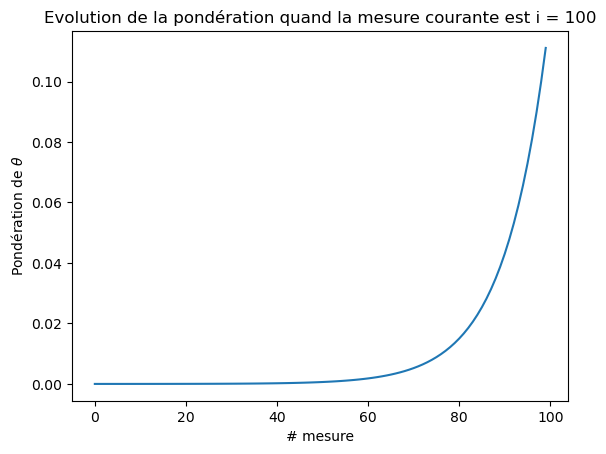
\includegraphics[width=1.0\linewidth]{Images/mep_decroissance}
				\label{fig:mep_decroissance}
			\end{figure}			
		\end{column}
		\begin{column}{0.5\textwidth}
			This visualization maps the geometric decay of historical weights evaluated from the standpoint of the 100\textsuperscript{th} step. The curve reveals the underlying power function of $\beta$, which gives this filtering strategy its formal designation as an \textbf{exponential} moving average.
		\end{column}	
	\end{columns}
\end{frame}

\begin{frame}{Tuning the Smoothness Window}
	\begin{columns}
		\begin{column}{0.5\textwidth}
			\begin{figure}
				\centering
				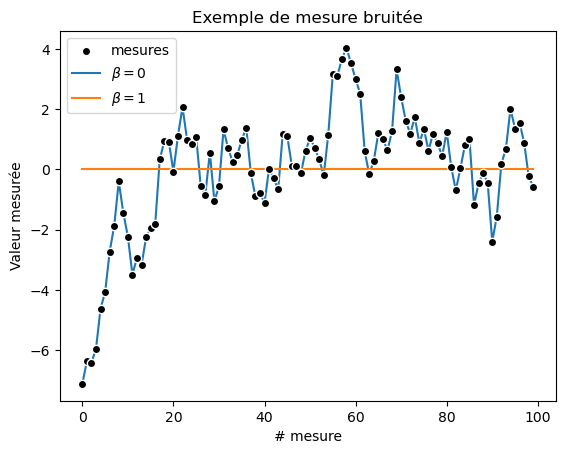
\includegraphics[width=1.0\linewidth]{Images/mesure_bruitee_extremes}
				\label{fig:mesure_bruitee_extremes}
			\end{figure}			
		\end{column}
		\begin{column}{0.5\textwidth}
			\begin{figure}
				\centering
				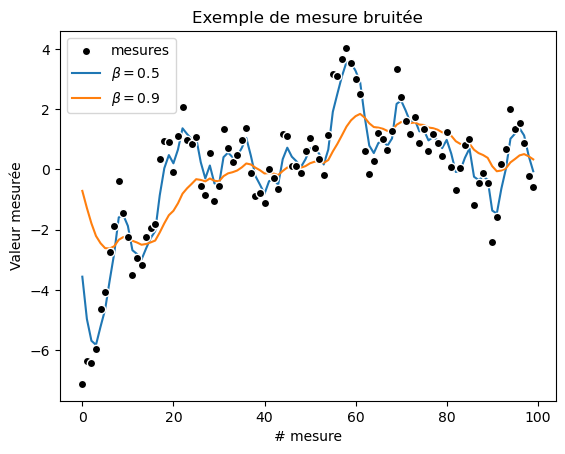
\includegraphics[width=1.0\linewidth]{Images/mesure_bruitee_raisonnable}
				\label{fig:mesure_bruitee_raisonnable}
			\end{figure}			
		\end{column}	
	\end{columns}
	\pause
	The impact of parameter $\beta$ on global smoothing is striking: as $\beta \to 1$, the filtering effect scales in power. However, a severe cold-start initialization anomaly becomes apparent during the earliest steps.
\end{frame}

\begin{frame}{Cold-Start Anomalies and Bias Correction}
	This initialization distortion is induced by the arbitrary setting $v^{(0)} = 0$. At the first step ($i = 1$):
	\begin{equation*}
		v^{(1)} = (1 - \beta) \theta_1 + \beta v^{(0)} = (1 - \beta) \theta_1
	\end{equation*}
	As $\beta \to 1$, the initial filtered estimate is heavily crushed toward zero. To correct this structural distortion, we introduce an exact analytical \textbf{bias correction} step:
	\pause
	\begin{equation*}
		\begin{cases}
			v^{(i)} = (1 - \beta) \theta_i + \beta v^{(i-1)} \\
			\hat{v}^{(i)} = \displaystyle \frac{v^{(i)}}{1 - \beta^i}
		\end{cases}
	\end{equation*}
	\pause
	At the first iteration ($i = 1$), the expression resolves exactly to: $\hat{v}^{(1)} = \theta_1$, completely neutralizing the initialization bias. As step index $i$ scales, the correction denominator $1 - \beta^i$ rapidly approaches 1, rendering the scaling factor neutral for later steps.
	
	\vspace{0.2cm}
	\textbf{Warning}: When compiling this algorithm in code, the recursive tracking loop must update the raw memory register $v$, not the bias-corrected output $\hat{v}$.
\end{frame}

\begin{frame}{The Complete Bias-Corrected EWMA Algorithm}
	Here is the formalized, robust algorithm incorporating dynamic bias correction:
	\begin{enumerate}
		\item Initialize the base filter register: $v = 0$.
		\item Set a target memory retention hyperparameter value for $\beta$.
		\item Loop sequentially across the $n$ data steps:
		\begin{itemize}
			\item Extract the current measurement: $\theta_i$.
			\item Compute the recursive update step: $v \leftarrow (1 - \beta) \theta_i + \beta v$.
			\item Execute the dynamic bias correction adjustment: $\hat{v} \leftarrow \frac{v}{1 - \beta^i}$.
		\end{itemize}
	\end{enumerate}
\end{frame}

\begin{frame}{Visualizing Bias Correction Impacts}
	These comparative plots demonstrate the tracking efficiency achieved via bias correction across separate configurations of $\beta$:
	\begin{columns}
		\begin{column}{0.5\textwidth}
			\begin{figure}
				\centering
				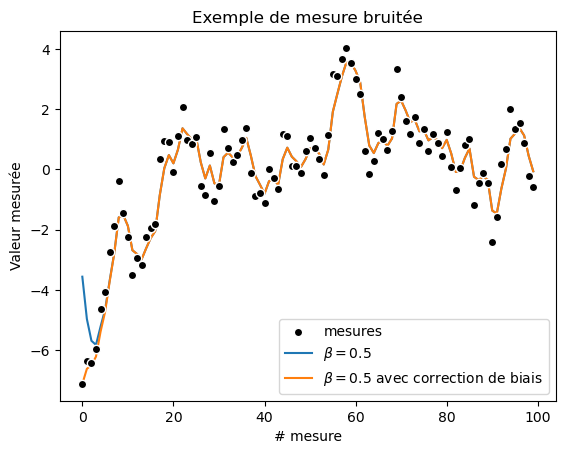
\includegraphics[width=1.0\linewidth]{Images/mesure_bruitee_biais1}
				\label{fig:mesure_bruitee_biais1}
			\end{figure}			
		\end{column}
		\begin{column}{0.5\textwidth}
			\begin{figure}
				\centering
				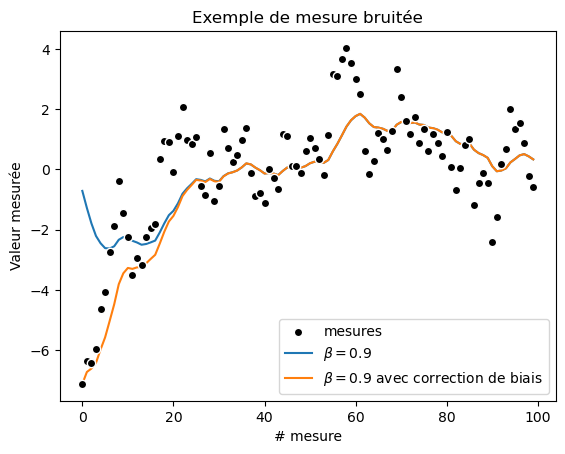
\includegraphics[width=1.0\linewidth]{Images/mesure_bruitee_biais2}
				\label{fig:mesure_bruitee_biais2}
			\end{figure}			
		\end{column}	
	\end{columns}
\end{frame}

\begin{frame}{Advanced Optimization Infrastructure}
	While computationally elementaire, this recursive filter is incredibly powerful when applied to machine learning optimization challenges:
	\begin{itemize}
		\item It is extremely \textbf{fast}: filtering requires only basic floating-point execution steps.
		\item It is highly efficient in \textbf{memory allocation}: a single variable completely encapsulates the network's history.
	\end{itemize}
	This mathematical engine is deployed to enhance standard gradient descent frameworks:
	\begin{itemize}
		\item By smoothing the directional \textbf{\textit{trajectory}} of updates (the first moment): the \textbf{Momentum} method.
		\item By scaling step magnitudes based on historical \textbf{\textit{oscillations}} (the second moment): the \textbf{RMSprop} algorithm.
		\item By unifiying structural trajectory and adaptive scaling: the industry standard \textbf{Adam} optimizer.
	\end{itemize}
\end{frame}

\subsection[Gradient Descent with Momentum]{Gradient Descent with Momentum}

\begin{frame}{Gradient Descent with Momentum}
	The gradient descent with Momentum framework, pioneered by Boris Polyak in 1964, filters stochastic trajectories by applying an exponential moving average directly to the computed \textbf{gradient vector}. We denote this memory tracking hyperparameter as $\beta_1$:
	\begin{enumerate}
		\item Initialize network parameter fields: $P$.
		\pause
		\item Initialize matching velocity tracking registers for each parameter: $v_P = 0$.
		\pause
		\item Loop across sequential training \textbf{epochs}.
		\pause
		\item For each mini-batch sample of volume $m$:
		\begin{itemize}
			\item Execute the forward pass and compute the current error cost $e$.
			\pause
			\item Backpropagate to evaluate the current raw gradient: $\nabla_P = \frac{\partial{e}}{\partial{P}}$.
			\pause
			\item Smooth the directional update trajectory: $v_P \leftarrow (1 - \beta_1) \nabla_P + \beta_1 v_P$.
			\pause 
			\item Execute parameter field updates: $P \leftarrow P - \alpha v_P$.
		\end{itemize}
		\item Return to Step 3 until specified stopping criteria are satisfied.
	\end{enumerate}	
\end{frame}

\begin{frame}{Momentum Optimization Trajectory}
	\begin{figure}
		\centering
		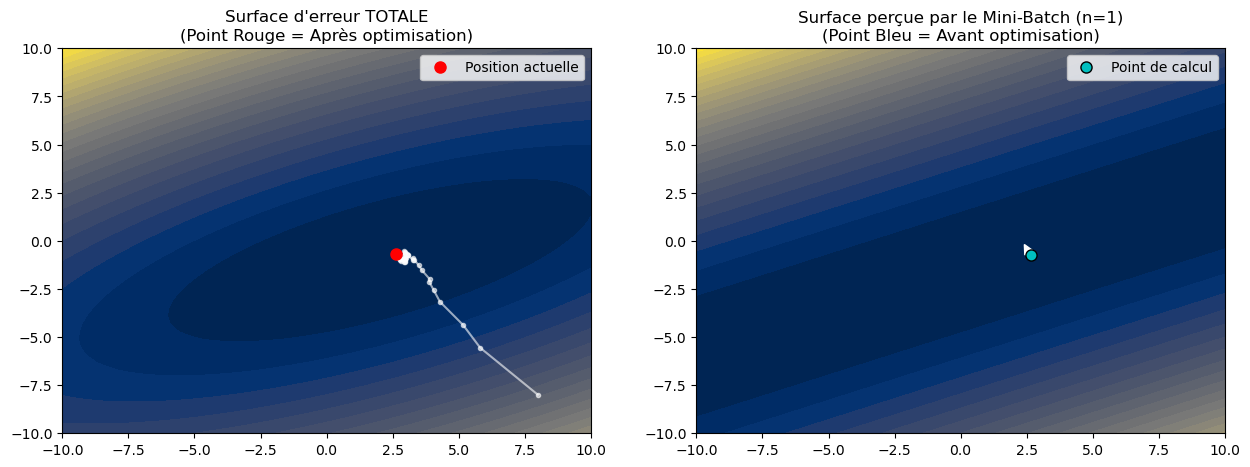
\includegraphics[height=0.35\linewidth]{Images/descente_gradient_momentum}
		\label{fig:descente_gradient_momentum}
	\end{figure}
	Note: Spatial dimensions trace the optimization updates across parameters $W$ and $b$ for a linear baseline: $\hat{Y} = X W + b$. Here, $\beta_1 = 0.9$, $m = 1$, and $\alpha = 0.1$.
\end{frame}

\subsection[The RMSprop Algorithm]{The RMSprop Algorithm}

\begin{frame}{The RMSprop Algorithm}
	The RMSprop (\textit{Root Mean Square Propagation}) algorithm applies an exponential moving average onto the \textbf{squared gradients}. During parameter updates, it \textbf{divides} the base learning step $\alpha \nabla_P$ element-wise by the square root of this historical moving average. This framework applies an \textbf{adaptive learning rate} localized per parameter:
	\pause
	\begin{itemize}
		\item Along coordinates exhibiting high variance and \textbf{large gradients}, step sizes are compressed to protect structural stability: propagation \textbf{decelerates}.
		\item Along coordinates exhibiting low variance and \textbf{small gradients}, step sizes are scaled up to accelerate search speed: propagation \textbf{accelerates}.
	\end{itemize}
	\pause
	Momentum minimizes time-to-convergence by smoothing directional trajectory paths, whereas RMSprop saves compute time by allowing the optimization loop to deploy a higher initial learning rate safely.
	
	\vspace{0.3cm}
	\pause
	The algorithm was introduced by Geoffrey Hinton in 2012 during his online lecture series. Hinton stands as a founding pioneer of connectionist deep learning.
\end{frame}

\begin{frame}{The RMSprop Algorithm}
	Let $\beta_2$ define the exponential memory coefficient tracking the squared gradient vectors. Let $\epsilon$ represent an infinitesimal regularization constant (typically $10^{-8}$) to prevent division-by-zero errors:
	\begin{enumerate}
		\item Initialize parameter fields: $P$.
		\pause
		\item Initialize matching squared-velocity tracking registers: $s_P = 0$.
		\pause
		\item Loop across sequential training \textbf{epochs}.
		\pause
		\item For each mini-batch sample of volume $m$:
		\begin{itemize}
			\item Compute the forward pass and resolve the current cost metric $e$.
			\pause
			\item Compute gradients via backpropagation: $\nabla_P = \frac{\partial{e}}{\partial{P}}$.
			\pause
			\item Accumulate the element-wise squared historical moving average: $s_P \leftarrow (1 - \beta_2) \nabla_P \odot \nabla_P + \beta_2 s_P$.
			\pause 
			\item Execute adaptive parameter updates: $P \leftarrow P - \frac{\alpha}{\sqrt{s_P} + \epsilon} \nabla_P$.
		\end{itemize}
		\item Return to Step 3.
	\end{enumerate}	
\end{frame}

\begin{frame}{RMSprop Optimization Trajectory}
	\begin{figure}
		\centering
		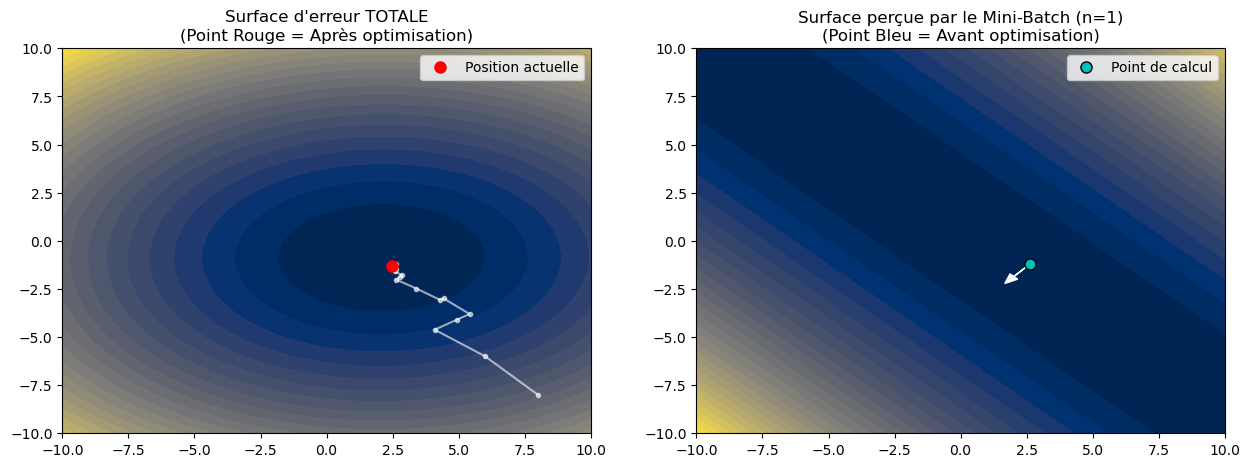
\includegraphics[height=0.35\linewidth]{Images/descente_gradient_rmsprop}
		\label{fig:descente_gradient_prop}
	\end{figure}
	Note: Spatial dimensions trace updates across parameters $W$ and $b$ for a linear baseline: $\hat{Y} = X W + b$, configured with $\beta_2 = 0.99$, $m = 1$, and $\alpha = 0.2$.
\end{frame}

\subsection[The Adam Optimizer]{The Adam Optimizer}

\begin{frame}{The Adam Optimizer}
	The \textbf{Adam} (\textit{Adaptive Moment Estimation}) optimization framework unifies the core strengths of both worlds: it fuses the trajectory smoothing of Momentum ($\beta_1$) with the adaptive coordinate scaling of RMSprop ($\beta_2$), while embedding rigorous structural \textbf{bias corrections}.
	
	\vspace{0.5cm}
	Engineered in 2014 by Diederik Kingma and Jimmy Ba, the seminal Adam publication stands as one of the most cited papers in the entire history of computer science and artificial intelligence.
\end{frame}

\begin{frame}{The Adam Algorithmic Steps}
	The complete formalized workflow for the Adam optimizer executes as follows:
	\begin{enumerate}
		\item Initialize matrix parameter fields: $P$.
		\item Initialize a global update step counter: $t = 0$.
		\item For each parameter, initialize moment tracking registers: $v_P = 0$ and $s_P = 0$.
		\item Loop across sequential training \textbf{epochs}.
		\item For each mini-batch sample of volume $m$:
		\begin{itemize}
			\item Increment the global step counter: $t \leftarrow t + 1$.
			\item Execute the forward pass and compute the current error cost $e$.
			\item Backpropagate to extract current gradients: $\nabla_P = \frac{\partial{e}}{\partial{P}}$.
			\item Track the 1\textsuperscript{st} moment (Momentum): $v_P \leftarrow (1 - \beta_1) \nabla_P + \beta_1 v_P$.
			\item Track the 2\textsuperscript{nd} moment (RMSprop): $s_P \leftarrow (1 - \beta_2) \nabla_P \odot \nabla_P + \beta_2 s_P$.
			\item Apply cold-start bias corrections: $\widehat{v_P} = v_P / (1 - \beta_1^t)$ and $\widehat{s_P} = s_P / (1 - \beta_2^t)$.
			\item Execute the final update step: $P \leftarrow P - \frac{\alpha}{\sqrt{\widehat{s_P}} + \epsilon} \widehat{v_P}$.
		\end{itemize}
		\item Return to Step 4.		
	\end{enumerate}	
\end{frame}

\begin{frame}{Adam Optimization Trajectory}
	\begin{figure}
		\centering
		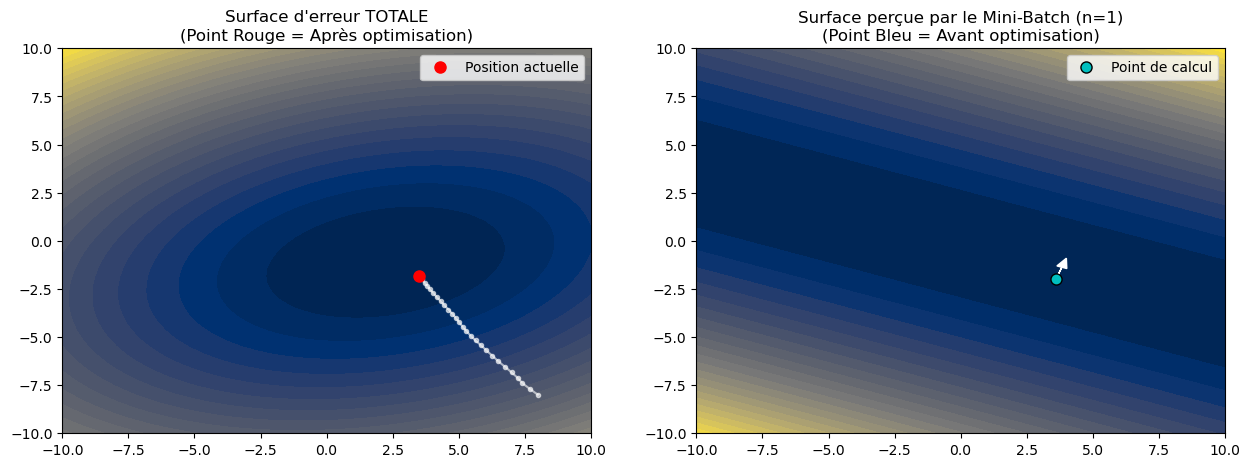
\includegraphics[height=0.35\linewidth]{Images/descente_gradient_adam}
		\label{fig:descente_gradient_adam}
	\end{figure}
	Note: Parameters $W$ and $b$ are optimized via Adam ($\beta_1 = 0.9$, $\beta_2 = 0.99$, $m = 1$, and $\alpha = 0.3$) for the linear system: $\hat{Y} = X W + b$.
\end{frame}

\subsection[Optimization Framework Conclusions]{Optimization Framework Conclusions}

\begin{frame}{Optimization Summary}
	We have analyzed three distinct paradigms engineered to optimize neural network parameter fields. By successfully tracking and balancing both 1\textsuperscript{st} and 2\textsuperscript{nd} order moments, \textbf{Adam} has become the undisputed \textbf{industry standard optimizer} for training deep connectionist topologies across a wide range of architectures.
	
	\pause
	\vspace{0.5cm}
	We have also demonstrated that the \textbf{batch size} hyperparameter $m$ balances a critical trade-off: maximizing hardware parallel processing efficiency via matrix vectorization without causing VRAM capacity overflows. Batch volume actively shapes the optimization trajectory, although Momentum filters out stochastic instability.
\end{frame}

\subsection[Weight Initialization and Gradient Stabilities]{Weight Initialization and Gradient Stabilities}

\begin{frame}{The Vanishing and Exploding Gradient Dilemma}
	Until now, we have assumed that parameter fields are simply initialized \textit{randomly}. In this section, we will define the exact mathematical logic governing this initialization. As neural topologies scale in depth, two pathologically destructive phenomena can paralyze backpropagation:
	\pause
	\begin{itemize}
		\item \textbf{Exploding Gradients}: If weight matrices are initialized with large values, the error signals are multiplied by factors greater than 1 at each layer. Gradients scale exponentially across depth, resulting in floating-point capacity failures (\textit{numerical overflow}).
		\pause
		\item \textbf{Vanishing Gradients}: Conversely, if weight fields are too small or if activation functions saturate, the error signal is multiplied by factors near 0 at each layer. The gradient effectively extinguishes before reaching the front layers of the network. Lacking gradient signals, these early feature extractors can never update their weights.
	\end{itemize}
\end{frame}

\begin{frame}{Mathematical Foundations: Variance Preservation}
	The solution to this architectural dilemma requires controlling the \textbf{variance} of layer activations and backpropagated gradients across the network topology via mathematically sound initialization bounds.
	
	\pause
	
	Consider an isolated linear transformation without bias: $Z = X W$, where $X \in \mathcal{M}_{n, u}(\R)$, $W \in \mathcal{M}_{u, v}(\R)$, and the output matrix is $Z \in \mathcal{M}_{n, v}(\R)$. We must guarantee that the variance of output states $Z$ matches the variance of input features $X$ to prevent signal decay or explosion.
	
	\pause
	
	Postulating that inputs and weights are mutually independent (zero covariance), zero-mean ($\E{X}=0, \E{W}=0$), and identically distributed, probability theory demonstrates that:
	\begin{equation*}
		\Var{Z^{(i)}_j} = u \cdot \Var{X^{(i)}_k} \cdot \Var{W_{k,j}}
	\end{equation*}
	
	\pause

	To enforce the variance identity constraint $\Var{Z^{(i)}_j} = \Var{X^{(i)}_k}$, we must scale the variance of our initialized weights such that:
	\begin{equation*}
		\Var{W_{k,j}} = \frac{1}{u}
	\end{equation*}
\end{frame}

\begin{frame}{Xavier / Glorot Initialization (Logistic and Tanh)}
	To accommodate the logistic function, Xavier Glorot and Yoshua Bengio (2010) formulated a balanced compromise that handles the variance constraints of both the forward pass ($n_{\text{in}}$) and the backward pass ($n_{\text{out}}$):
	
	\begin{block}{Xavier / Glorot Initialization (Logistic Curves)}
		For a network layer feeding from $n_{\text{in}}$ inputs to $n_{\text{out}}$ output nodes, weight matrices are sampled from a centered Gaussian distribution:
		\begin{equation*}
			W_{i,j} \sim \mathcal{N}\left(0, \, \sigma^2\right) \quad \text{with} \quad \sigma = \sqrt{\frac{2}{n_{\text{in}} + n_{\text{out}}}}
		\end{equation*}
		Or sampled from a bounded uniform distribution:
		\begin{equation*}
			W_{i,j} \sim \mathcal{U}\left(-\sqrt{\frac{6}{n_{\text{in}} + n_{\text{out}}}}, \, \sqrt{\frac{6}{n_{\text{in}} + n_{\text{out}}}}\right)
		\end{equation*}
		
		\vspace{-0.2cm}
		
		Both structural distributions map to the exact same theoretical variance: $\frac{2}{n_{\text{in}} + n_{\text{out}}}$.
	\end{block}
\end{frame}

\begin{frame}{Xavier Initialization for Logistic Layers}
	\begin{columns}
		\begin{column}{0.65\textwidth}
			\begin{figure}
				\centering
				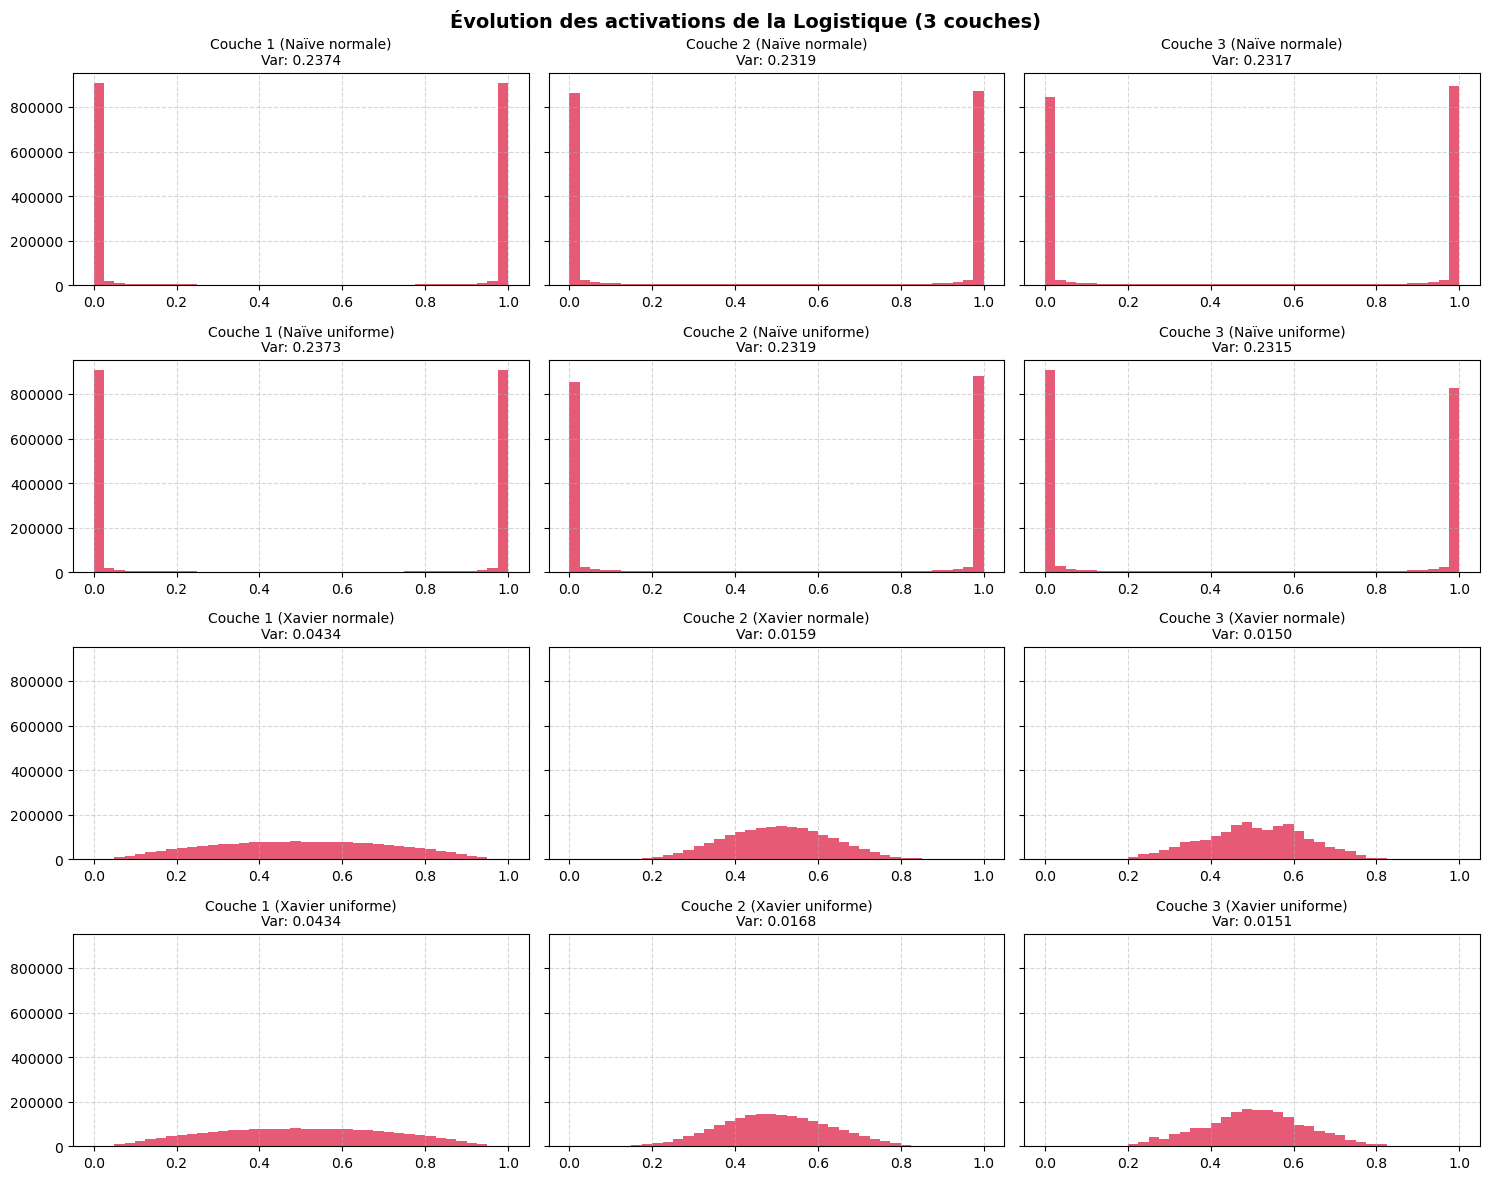
\includegraphics[width=1.0\linewidth]{Images/xavier_logistique}
				\label{fig:xavier_logistique}
			\end{figure}				
		\end{column}
		\begin{column}{0.35\textwidth}
			Deploying a naive initialization strategy (e.g., standard unit variance) saturates the logistic function immediately. Local gradients flatline to zero, paralyzing the optimization loop.
			
			\vspace{0.2cm}
			
			Even when calibrated via Xavier initialization, logistic hidden nodes cause a steady decay in signal variance. Consequently, the logistic curve has been phased out of hidden layers.
		\end{column}
	\end{columns}
\end{frame}

\begin{frame}{Xavier / Glorot Initialization (Logistic and Tanh)}
	When handling the hyperbolic tangent activation function, an explicit scaling gain modifier $\gamma = \frac{5}{3}$ is integrated to correct for the impact of non-linear curvature on variance tracking:
	
	\begin{block}{Xavier / Glorot Initialization (Tanh Activations)}
		Given a hidden layer topology spanning $n_{\text{in}}$ inputs and $n_{\text{out}}$ outputs, parameter fields are drawn from a Gaussian distribution:
		\begin{equation*}
			W_{i,j} \sim \mathcal{N}\left(0, \, \sigma^2\right) \quad \text{with} \quad \sigma = \gamma \sqrt{\frac{2}{n_{\text{in}} + n_{\text{out}}}}
		\end{equation*}
		Or drawn from its uniform counterpart:
		\begin{equation*}
			W_{i,j} \sim \mathcal{U}\left(-\gamma \sqrt{\frac{6}{n_{\text{in}} + n_{\text{out}}}}, \,  \gamma \sqrt{\frac{6}{n_{\text{in}} + n_{\text{out}}}}\right)
		\end{equation*}
		The optimized target initialization variance evaluates to: $\frac{2 \gamma^2}{n_{\text{in}} + n_{\text{out}}}$.
	\end{block}
\end{frame}

\begin{frame}{Xavier Initialization for Tanh Layers}
	\begin{columns}
		\begin{column}{0.65\textwidth}
			\begin{figure}
				\centering
				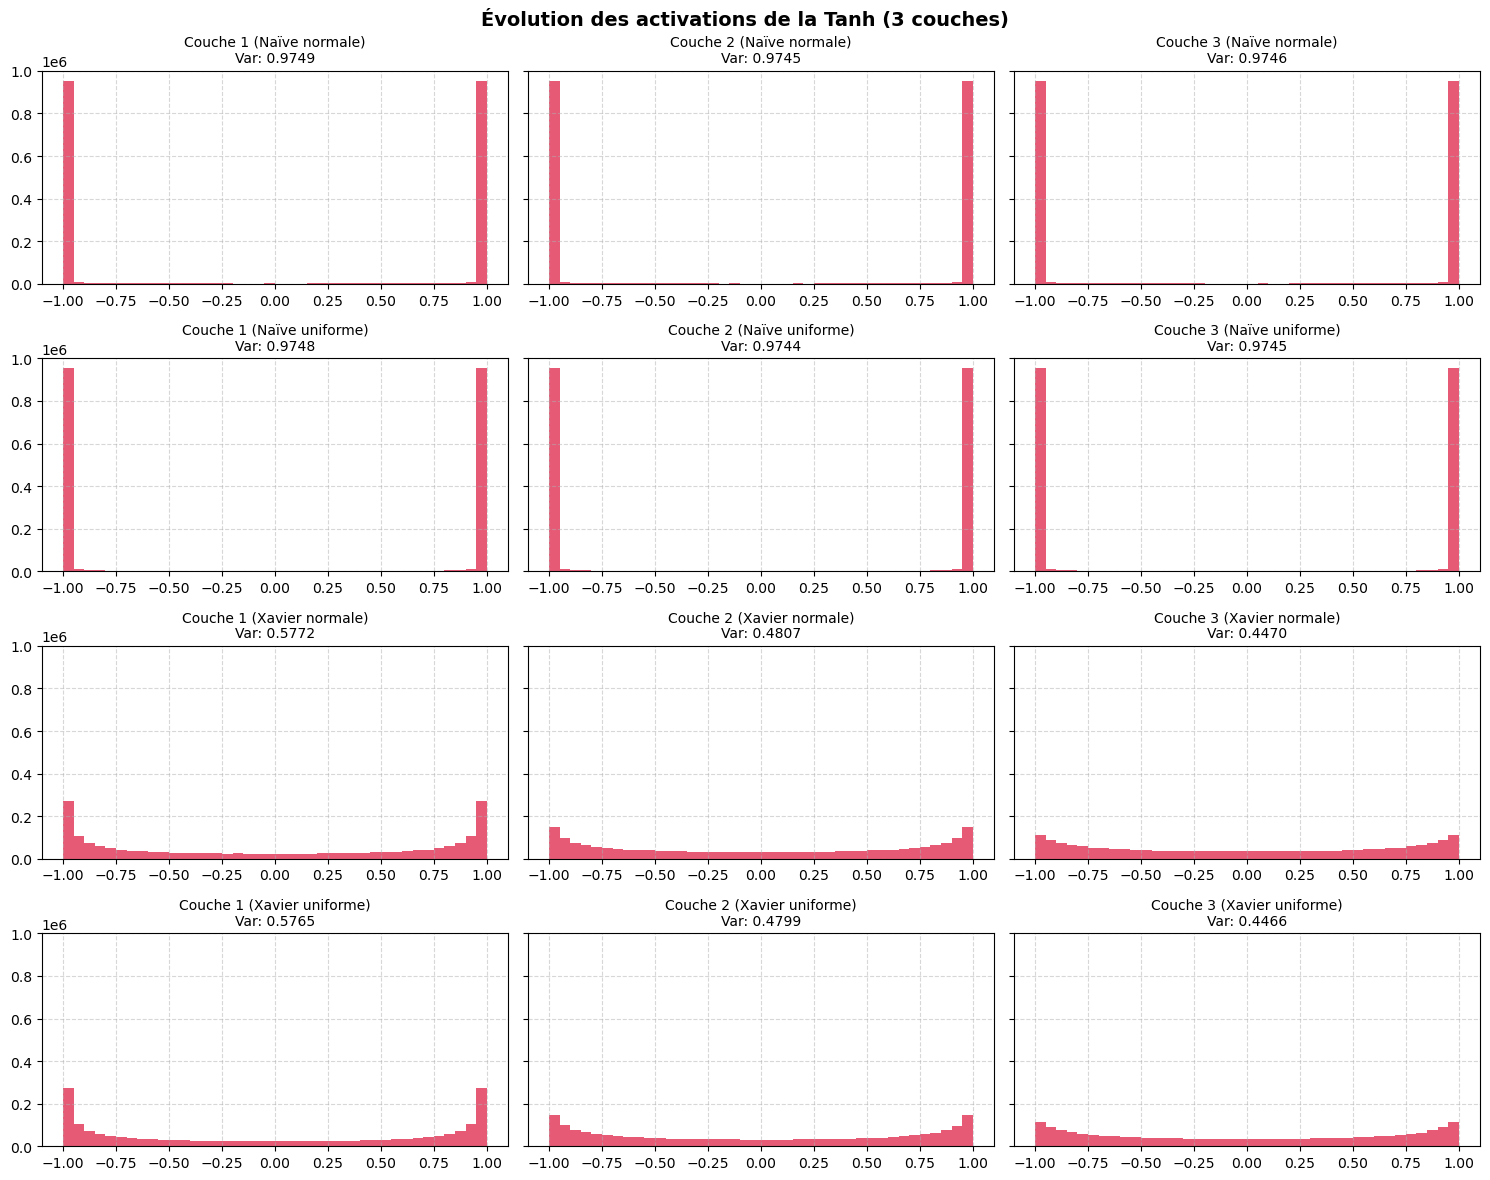
\includegraphics[width=1.0\linewidth]{Images/xavier_tanh}
				\label{fig:xavier_tanh}
			\end{figure}				
		\end{column}
		\begin{column}{0.35\textwidth}
			A naive unit-variance initialization scheme causes identical saturation failures when applied to hyperbolic tangent layers.
			
			\vspace{0.5cm}
			Implementing the Xavier framework maintains a stable equilibrium: it eliminates saturation zones and prevents the collapse of signal variance across layers.
		\end{column}
	\end{columns}
\end{frame}

\begin{frame}{Kaiming / He Initialization (ReLU)}
	The Rectified Linear Unit function $\operatorname{ReLU}(Z) = \max(0, Z)$ breaks the fundamental symmetry assumptions of classical initialization: it completely truncates and sets to zero exactly 50\% of its input space on average. As a result, the forward signal loses half its variance at every layer!
	
	\vfill
	\pause
	To compensate for this systematic loss of signal variance, Kaiming He (2015) demonstrated that the initialization variance assigned to the weights must be doubled compared to the Xavier model.
\end{frame}

\begin{frame}{Kaiming / He Initialization (ReLU)}
	\begin{block}{Kaiming / He Initialization Framework}
		For a deep network layer utilizing ReLU activation nodes driven by $n_{\text{in}}$ input connections, parameter fields are generated from a centered Gaussian distribution:
		\begin{equation*}
			W_{i,j} \sim \mathcal{N}\left(0, \, \sigma^2\right) \quad \text{with} \quad \sigma = \sqrt{\frac{2}{n_{\text{in}}}}
		\end{equation*}	
		Or generated from its equivalent uniform bounded distribution:
		\begin{equation*}
			W_{i,j} \sim \mathcal{U}\left(-\sqrt{\frac{6}{n_{\text{in}}}}, \, \sqrt{\frac{6}{n_{\text{in}}}}\right)
		\end{equation*}
		The stabilizing target variance is calibrated to evaluate exactly as: $\frac{2}{n_{\text{in}}}$.
	\end{block}
\end{frame}

\begin{frame}{Kaiming Initialization for ReLU Layers}
	\begin{columns}
		\begin{column}{0.65\textwidth}
			\begin{figure}
				\centering
				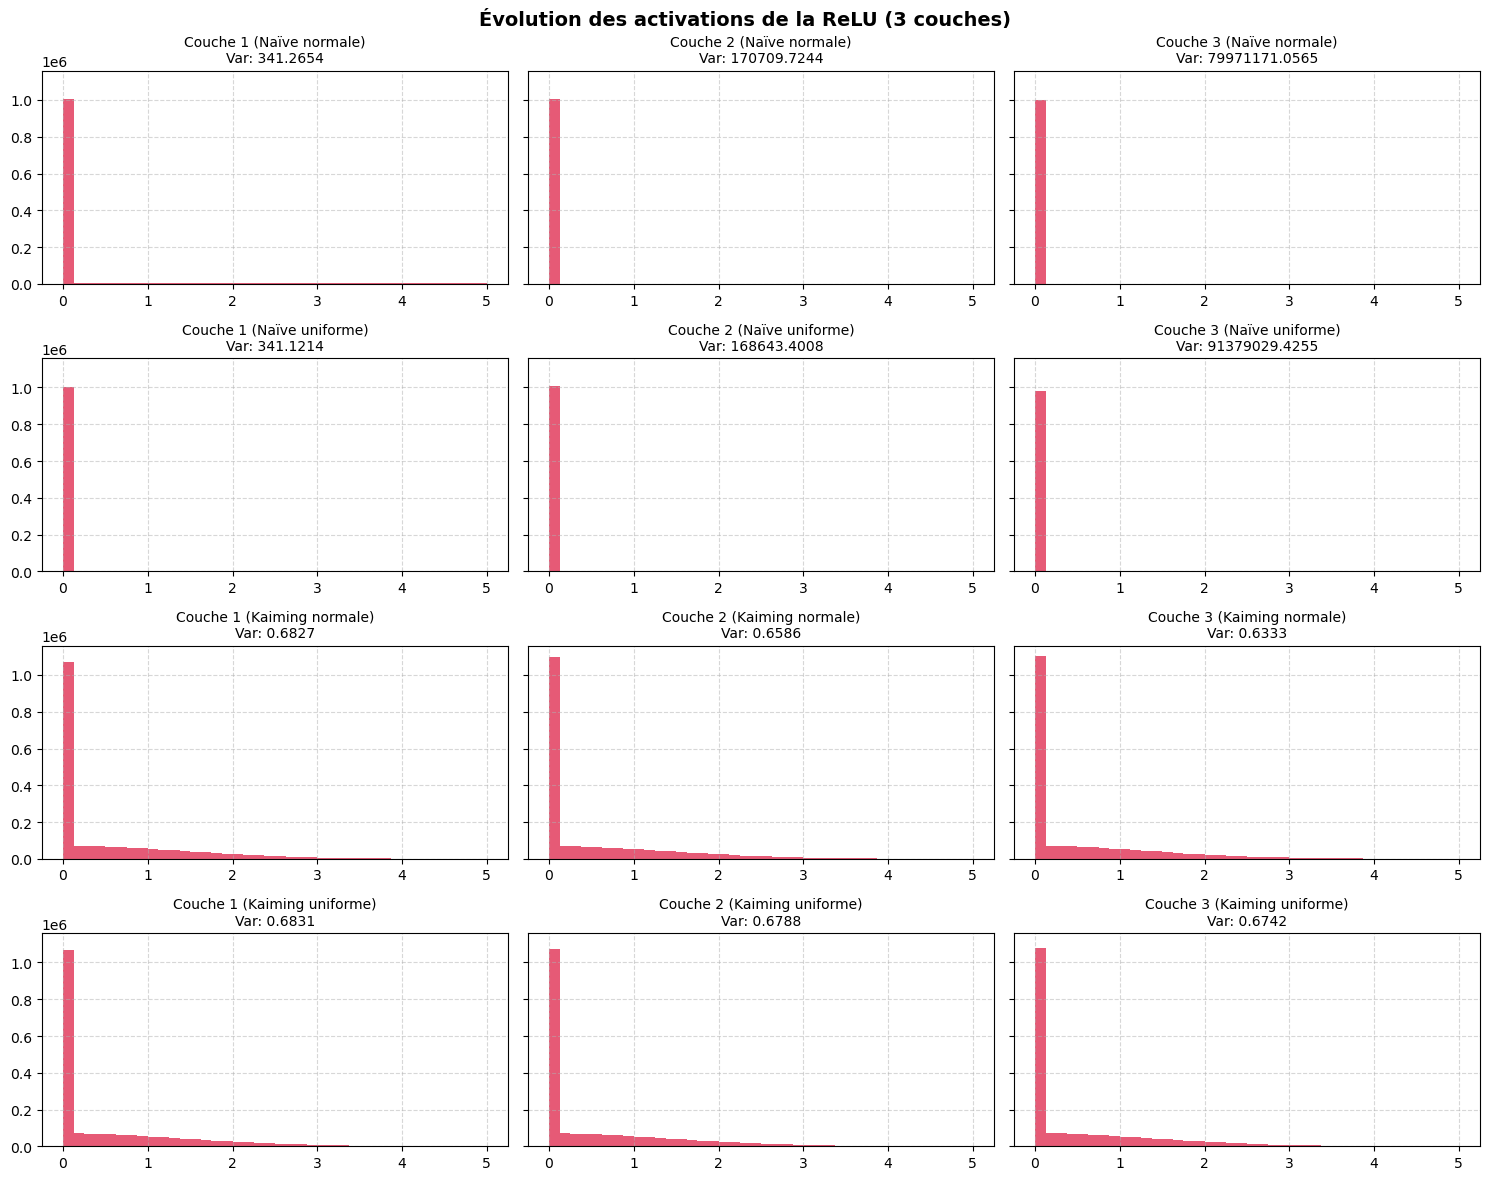
\includegraphics[width=1.0\linewidth]{Images/kaiming_relu}
				\label{fig:kaiming_relu}
			\end{figure}				
		\end{column}
		\begin{column}{0.35\textwidth}
			Deploying a naive initialization scheme here triggers a destructive asymmetry: it causes absolute signal extinction for half the neurons, while driving an explosive, exponential inflation of variance across the remaining active pathways.
			
			\vspace{0.5cm}
			The Kaiming He initialization protocol neutralizes this truncation effect, keeping the signal variance stable across deep layers.
		\end{column}
	\end{columns}
\end{frame}

\begin{frame}{Initialization Strategy Conclusions}
	Rigorous weight initialization calibration is a necessary mathematical condition to prevent gradient explosion or decay during the cold-start phase of training. However, it cannot guarantee stability throughout the entire optimization process.
	
	\pause
	\vspace{0.5cm}
	Initialization protocols are paired with strategic activation functions (such as ReLU for deep topologies) and advanced architectural scaling methodologies, such as Batch Normalization. Furthermore, deep residual network topologies (\textit{ResNets}) deploy shortcut connections specifically designed to route gradient signals unimpeded across more than 1,000 layers.
	
	\pause
	\vspace{0.3cm}
	Note: Structural bias vectors do not require variance tracking; they are simply initialized to 0 in the vast majority of deep learning architectures.
\end{frame}

\subsection[Conclusions]{Conclusions}

\begin{frame}{Optimization Review}
	In this comprehensive section, we have formalized the complete mathematical and operational toolkit required to orchestrate parameter updates across neural network architectures:
	\begin{itemize}
		\item We defined specialized \textbf{loss functions} tailored to targeted supervised frameworks: Mean-Squared Error (MSE) for regression, and Binary/Categorical Cross-Entropy for classification tasks.
		\item We mastered the analytical fusion techniques engineered to maximize performance by collapsing the final activation layer and loss derivatives into a highly stable, efficient expression.
	\end{itemize}
\end{frame}

\begin{frame}{Optimization Review}
	\begin{itemize}
		\item We implemented and evaluated three distinct gradient descent optimization algorithms:
		\begin{itemize}
			\item The \textbf{Momentum} framework to filter stochastic noise and guide update trajectories.
			\item The \textbf{adaptive learning rate} paradigm (RMSprop) to regulate coordinate step sizes and ensure numerical stability.
			\item The industry-standard unified optimizer: \textbf{Adam}.
		\end{itemize}
		\item Finally, we formalized variance tracking using the initialization frameworks of \textbf{Xavier/Glorot} and \textbf{Kaiming/He}, neutralizing the risks of vanishing or exploding gradients.
	\end{itemize}
\end{frame}